\documentclass[aspectratio=43]{beamer}
\usepackage[
    backend=biber,
    style=authoryear,
  ]{biblatex}


% Title --------------------------------------------
\title{LLMs: Applications to Economics Research}
\date{\today}
\author{Nathan Williams}
% xcolor and define colors -------------------------
\usepackage{xcolor}
\usepackage[fleqn]{amsmath}

% https://www.viget.com/articles/color-contrast/
\definecolor{purple}{HTML}{695693}
\definecolor{navy}{HTML}{567293}
\definecolor{ruby}{HTML}{9a2515}
\definecolor{alice}{HTML}{107895}
\definecolor{daisy}{HTML}{EBC944}
\definecolor{coral}{HTML}{F26D21}
\definecolor{kelly}{HTML}{829356}
\definecolor{cranberry}{HTML}{E64173}
\definecolor{jet}{HTML}{131516}
\definecolor{asher}{HTML}{555F61}
\definecolor{slate}{HTML}{314F4F}

% Main theme colors
\definecolor{accent}{HTML}{107895}
\definecolor{accent2}{HTML}{9a2515}


\newcommand\navy[1]{{\color{navy}#1}}
\newcommand\purple[1]{{\color{purple}#1}}
\newcommand\kelly[1]{{\color{kelly}#1}}
\newcommand\ruby[1]{{\color{ruby}#1}}
\newcommand\alice[1]{{\color{alice}#1}}
\newcommand\daisy[1]{{\color{daisy}#1}}
\newcommand\coral[1]{{\color{coral}#1}}
\newcommand\cranberry[1]{{\color{cranberry}#1}}
\newcommand\slate[1]{{\color{slate}#1}}
\newcommand\jet[1]{{\color{jet}#1}}
\newcommand\asher[1]{{\color{asher}#1}}

\newcommand\bgNavy[1]{{\colorbox{navy!80!white}{#1}}}
\newcommand\bgPurple[1]{{\colorbox{purple!80!white}{#1}}}
\newcommand\bgKelly[1]{{\colorbox{kelly!80!white}{#1}}}
\newcommand\bgRuby[1]{{\colorbox{ruby!80!white}{#1}}}
\newcommand\bgAlice[1]{{\colorbox{alice!80!white}{#1}}}
\newcommand\bgDaisy[1]{{\colorbox{daisy!80!white}{#1}}}
\newcommand\bgCoral[1]{{\colorbox{coral!80!white}{#1}}}
\newcommand\bgCranberry[1]{{\colorbox{cranberry!80!white}{#1}}}


% Beamer Options -------------------------------------

% Background
\setbeamercolor{background canvas}{bg = white}

% Change text margins
\setbeamersize{text margin left = 15pt, text margin right = 15pt} 

% \alert
\setbeamercolor{alerted text}{fg = accent2}

% Frame title
\setbeamercolor{frametitle}{bg = white, fg = jet}
\setbeamercolor{framesubtitle}{bg = white, fg = accent}
\setbeamerfont{framesubtitle}{size = \small, shape = \itshape}

% Block
\setbeamercolor{block title}{fg = white, bg = accent2}
\setbeamercolor{block body}{fg = jet, bg = jet!10!white}

% Title page
\setbeamercolor{title}{fg = jet}
\setbeamercolor{subtitle}{fg = accent}

%% Custom \maketitle and \titlepage
\setbeamertemplate{title page}
{
    %\begin{centering}
        \vspace{20mm}
        {\Large \usebeamerfont{title}\usebeamercolor[fg]{title}\inserttitle}\\ \vskip0.25em%
        \ifx\insertsubtitle\@empty%
        \else%
          {\usebeamerfont{subtitle}\usebeamercolor[fg]{subtitle}\insertsubtitle\par}%
        \fi% 
        {\vspace{10mm}\insertauthor}\\
        {\color{asher}\small{\insertdate}}\\
    %\end{centering}
}

% Table of Contents
\setbeamercolor{section in toc}{fg = accent!70!jet}
\setbeamercolor{subsection in toc}{fg = jet}

% Button 
\setbeamercolor{button}{bg = accent}

% Remove navigation symbols
\setbeamertemplate{navigation symbols}{}

% Table and Figure captions
\setbeamercolor{caption}{fg=jet!70!white}
\setbeamercolor{caption name}{fg=jet}
\setbeamerfont{caption name}{shape = \itshape}

% Bullet points

%% Fix left-margins
\settowidth{\leftmargini}{\usebeamertemplate{itemize item}}
\addtolength{\leftmargini}{\labelsep}

%% enumerate item color
\setbeamercolor{enumerate item}{fg = accent}
\setbeamerfont{enumerate item}{size = \small}
\setbeamertemplate{enumerate item}{\insertenumlabel.}

%% itemize
\setbeamercolor{itemize item}{fg = accent!70!white}
\setbeamerfont{itemize item}{size = \small}
\setbeamertemplate{itemize item}[circle]

%% right arrow for subitems
\setbeamercolor{itemize subitem}{fg = accent!60!white}
\setbeamerfont{itemize subitem}{size = \small}
\setbeamertemplate{itemize subitem}{$\rightarrow$}

\setbeamertemplate{itemize subsubitem}[square]
\setbeamercolor{itemize subsubitem}{fg = jet}
\setbeamerfont{itemize subsubitem}{size = \small}

% References

%% Bibliography Font, roughly matching aea
\setbeamerfont{bibliography item}{size = \footnotesize}
\setbeamerfont{bibliography entry author}{size = \footnotesize, series = \bfseries}
\setbeamerfont{bibliography entry title}{size = \footnotesize}
\setbeamerfont{bibliography entry location}{size = \footnotesize, shape = \itshape}
\setbeamerfont{bibliography entry note}{size = \footnotesize}

\setbeamercolor{bibliography item}{fg = jet}
\setbeamercolor{bibliography entry author}{fg = accent!60!jet}
\setbeamercolor{bibliography entry title}{fg = jet}
\setbeamercolor{bibliography entry location}{fg = jet}
\setbeamercolor{bibliography entry note}{fg = jet}

%% Remove bibliography symbol in slides
\setbeamertemplate{bibliography item}{}





% Links ----------------------------------------------

\usepackage{hyperref}
\hypersetup{
  colorlinks = true,
  linkcolor = accent2,
  filecolor = accent2,
  urlcolor = accent2,
  citecolor = accent2,
}


% Line spacing --------------------------------------
\usepackage{setspace}
\setstretch{1.3}


% \begin{columns} -----------------------------------
\usepackage{multicol}

% \begin{mathematics} -------------------------------
\usepackage{amsmath}


% Fonts ---------------------------------------------
% Beamer Option to use custom fonts
\usefonttheme{professionalfonts}

% \usepackage[utopia, smallerops, varg]{newtxmath}
% \usepackage{utopia}
\usepackage[sfdefault,light]{roboto}

% Small adjustments to text kerning
\usepackage{microtype}



% Remove annoying over-full box warnings -----------
\vfuzz2pt 
\hfuzz2pt


% Table of Contents with Sections
\setbeamerfont{myTOC}{series=\bfseries, size=\Large}
\AtBeginSection[]{
        \frame{
            \frametitle{Roadmap}
            \tableofcontents[current]   
        }
    }


% References ----------------------------------------
\usepackage[
    citestyle= authoryear,
    style = authoryear,
    natbib = true, 
    backend = biber
]{biblatex}

% Smaller font-size for references
\renewcommand*{\bibfont}{\small}

% Remove "In:"
\renewbibmacro{in:}{}

% Color citations for slides
\newenvironment{citecolor}
    {\footnotesize\begin{color}{accent2}}
    {\end{color}}

\newcommand{\citetcolor}[1]{{\footnotesize\textcolor{gray}{\citet{#1}}}}
\newcommand{\citepcolor}[1]{{\footnotesize\textcolor{gray}{\citep{#1}}}}

% Tables -------------------------------------------
% Tables too big
% \begin{adjustbox}{width = 1.2\textwidth, center}
\usepackage{adjustbox}
\usepackage{array}
\usepackage{threeparttable, booktabs, adjustbox}
    
% Fix \input with tables
% \input fails when \\ is at end of external .tex file

\makeatletter
\let\input\@@input
\makeatother

% Tables too narrow
% \begin{tabularx}{\linewidth}{cols}
% col-types: X - center, L - left, R -right
% Relative scale: >{\hsize=.8\hsize}X/L/R
\usepackage{tabularx}
\newcolumntype{L}{>{\raggedright\arraybackslash}X}
\newcolumntype{R}{>{\raggedleft\arraybackslash}X}
\newcolumntype{C}{>{\centering\arraybackslash}X}

% Figures

% \imageframe{img_name} -----------------------------
% from https://github.com/mattjetwell/cousteau
\newcommand{\imageframe}[1]{%
    \begin{frame}[plain]
        \begin{tikzpicture}[remember picture, overlay]
            \node[at = (current page.center), xshift = 0cm] (cover) {%
                \includegraphics[keepaspectratio, width=\paperwidth, height=\paperheight]{#1}
            };
        \end{tikzpicture}
    \end{frame}%
}

% subfigures
\usepackage{subfigure}


% Highlight slide -----------------------------------
% \begin{transitionframe} Text \end{transitionframe}
% from paulgp's beamer tips
\newenvironment{transitionframe}{
    \setbeamercolor{background canvas}{bg=accent!60!black}
    \begin{frame}\color{accent!10!white}\LARGE\centering
}{
    \end{frame}
}


% Table Highlighting --------------------------------
% Create top-left and bottom-right markets in tabular cells with a unique matching id and these commands will outline those cells
\usepackage[beamer,customcolors]{hf-tikz}
\usetikzlibrary{calc}
\usetikzlibrary{fit,shapes.misc}

% To set the hypothesis highlighting boxes red.
\newcommand\marktopleft[1]{%
    \tikz[overlay,remember picture] 
        \node (marker-#1-a) at (0,1.5ex) {};%
}
\newcommand\markbottomright[1]{%
    \tikz[overlay,remember picture] 
        \node (marker-#1-b) at (0,0) {};%
    \tikz[accent!80!jet, ultra thick, overlay, remember picture, inner sep=4pt]
        \node[draw, rectangle, fit=(marker-#1-a.center) (marker-#1-b.center)] {};%
}
\begin{document}
%---------------------------------------------------
\begin{frame}
\maketitle
\end{frame}
%---------------------------------------------------
\section{Introduction}
%---------------------------------------------------
\begin{frame}{Why are we talking about AI and Research?}
    The proliferation of AI applications and Large Language Models for academic research has increased drastically in the schools.
    \begin{figure}
        \centering
        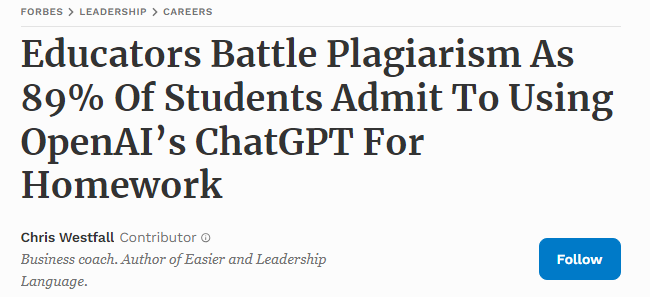
\includegraphics{News Screeenshot 1.png}
        \label{News Article}
    \end{figure}
\end{frame}
%-------------------------------------------------
\begin{frame}{Professors are having trouble too!}
    
\end{frame}
%-------------------------------------------------
\begin{frame}{Artificial Intelligence Platforms}
    The popularity of ChatGPT and OpenAI has led to the proliferation of many AI platforms
    \begin{itemize}
        \item Llama (Meta Product)
        \item StableLM
        \item Pythia
        \item BloombergGPT
    \end{itemize}
    This space is growing so quickly that there will likely be one announced over the course of this presentation.
\end{frame}
%------------------------------------------------
\begin{frame}{Using AI in Research}
    Using generated work in research can be very dangerous for the following reasons:
    \begin{itemize}
        \item Incorrect Information
        \item Plagiarism
    \end{itemize}
    The goal of this talk is to minimize the risks of either of these issues arising. 
\end{frame}
%----------------------------------------------
\begin{frame}{Skills Covered Here}
    Key applications will be covered in this lecture with respect to two skills:
    \begin{itemize}
        \item Coding
        \item Writing
    \end{itemize}
    This lecture will focus on using ChatGPT, but this can be broadly applied.
\end{frame}
%-----------------------------------------------
\section{General Rules of Thumb}
%-----------------------------------------------
\begin{frame}{General Rule of Thumb}\label{Rule of Thumb}
    LLMs tend to do worse at generating original material, as they tend to make things up if not properly prompted.
    \bigbreak 
    \begin{block}{Rule of Thumb}
        Avoid having an LLM generate its own work, use it to enhance your already existing work
    \end{block}
\end{frame}
%-----------------------------------------------
\begin{frame}{Construction of Queries}
    Every time a query is constructed, think of choosing a set of additional information such that the probability of a correct answer is maximized. There are a few key aspects that consistently improve the outputs of LLMs. 
    \begin{itemize}
        \item Writing clear text
        \item Prompt Structure
    \end{itemize}
\end{frame}
%----------------------------------------------
\begin{frame}{Basic Prompt Structure (\href{https://www.promptingguide.ai/introduction/basics}{Source})}\label{Prompt Structure}
    A well-structured prompt can have up to 4 key elements. These are not all needed but can be valuable in answering more complicated questions. 
    \begin{itemize}
        \item Instruction
        \item Context
        \item Input Data
        \item Output Data
    \end{itemize}
\end{frame}
%-----------------------------------------------
\begin{frame}{Some Other Key Prompt Approaches (\href{https://www.promptingguide.ai/introduction/basics}{Source})}
    Many of the standard rules of thumb for Google searches often apply here:
    \begin{itemize}
        \item Specificity
        \item Start Smaller
        \item Avoid Impreciseness
    \end{itemize}
\end{frame}
%-----------------------------------------------
\section{Coding}
%-----------------------------------------------
\begin{frame}{Coding in LLMs}
    The largest efficiency gain for researchers comes from LLM's coding ability. 
    \begin{itemize}
        \item Writing Code
        \item Interpreting Errors
        \item Streamlining Speed
    \end{itemize}
\end{frame}
%-----------------------------------------------
\begin{frame}{LLMs are not equally helpful}
    \begin{figure}
        \centering
        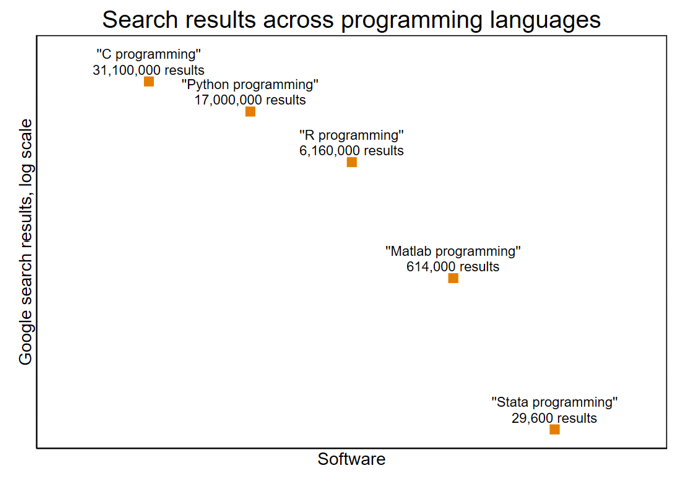
\includegraphics{Availability of Results on Internet.png}
    \end{figure}
\end{frame}
%-----------------------------------------------
\begin{frame}{Interpreting Errors}
    One of the most powerful tools LLMs can be used for is interpreting errors. Simply copy and paste your error into the interface window.

    \bigbreak 
    This is not a substitute to StackOverflow, but rather a compliment.
\end{frame}
%-----------------------------------------------
\begin{frame}{Prompt Strategy - Interpreting and Fixing Errors}
    A better way to interpret errors can be borrowed from the \alert{prompt engineering} literature:
    \begin{enumerate}
        \item Set up the \hyperlink{Prompt Structure}{prompting environment}
        \item Include both your code and your error
        \item Ask the LLM to explain the error in the context of your code in the \alert{Output Data} section
    \end{enumerate}
\end{frame}
%-----------------------------------------------
\begin{frame}{Streamlining Speed}
    In every subfield of economics, there exists simulations that can take a very long time (days to weeks). Small coding optimizations can take a project that takes weeks to simulate and move it to days. 
    \begin{itemize}
        \item Microeconomics (Bootstrapping)
        \item Macroeconomics (Model Estimation)
        \item Econometrics (Bootstrapping)
    \end{itemize}
    \bigbreak 
    ChatGPT and other LLMs are very good at finding these tiny optimizations! 
\end{frame}
%-----------------------------------------------
\begin{frame}{Prompt Strategy - Speeding Up Code}
    \begin{enumerate}
        \item Set up the \hyperlink{Prompt Structure}{prompting environment}
        \item Include your code in the \alert{Context} section
        \item Ask the LLM to find ways to optimize your code
    \end{enumerate}
\end{frame}
%-----------------------------------------------
\begin{frame}{Generating New Code}
    Per the \hyperlink{Rule of Thumb}{Rule of Thumb Slide}, it is a good idea to avoid an LLM generating all code for a few key reasons:
    \begin{itemize}
        \item The LLM may hallucinate packages or commands, especially as the program has less active resources on the internet (read: \alert{Stata}) 
        \item The prompt and structure must be very specific
        \item You still have to know what the code does! 
        \item Certain people may construe this as academic dishonesty
    \end{itemize}
    \alert{It is in your best interest not to do this.}
\end{frame}
%-----------------------------------------------
\section{Writing}
%-----------------------------------------------
\begin{frame}{LLMs are editors, not writers}
    Unlike with code, using an LLM to write for you is \alert{academic dishonesty} and you should not do it ever. 

    \bigbreak
    However, there are some uses for ChatGPT with writing that are both largely permissible and can serve to help you in your own writing.
\end{frame}
%----------------------------------------------
\begin{frame}{Why use an LLM to edit work?}
    One of the most popular strategies of editing is reading your work aloud to a friend (or yourself, no judgement). 
    This helps discern the quirks of your \alert{voice} that you otherwise might not see.

    \bigbreak
    If you don't have friends, ChatGPT and other LLMs can serve this purpose.
\end{frame}
%----------------------------------------------
\begin{frame}{Prompt Strategy - Editing Documents}
    \begin{itemize}
        \item Set up the \alert{prompting environment}, make sure the LLM knows it is an editor and not a writer
        \item Paste a section of the document that you would like to be edited and ask ChatGPT to edit it
    \end{itemize}
\end{frame}
%----------------------------------------------
\section{Conclusion}
%----------------------------------------------
\begin{frame}{LLMs and ChatGPT}
    Both are powerful, but dangerous tools in the research process. Please use caution when using. 
    \bigbreak
    
    If you have any questions, come see Hanna or Nathan and we will help you :)
\end{frame}
%----------------------------------------------
\end{document}